\documentclass{article}
\usepackage{booktabs}
\usepackage{graphicx}
\usepackage{geometry}
\usepackage{caption}
\usepackage{float}
\geometry{margin=1in}

\begin{document}

\section*{Churro Fine-Tuning Evaluation: Coverage and Semantic Error Rate}

\begin{figure}[H]
  \centering
  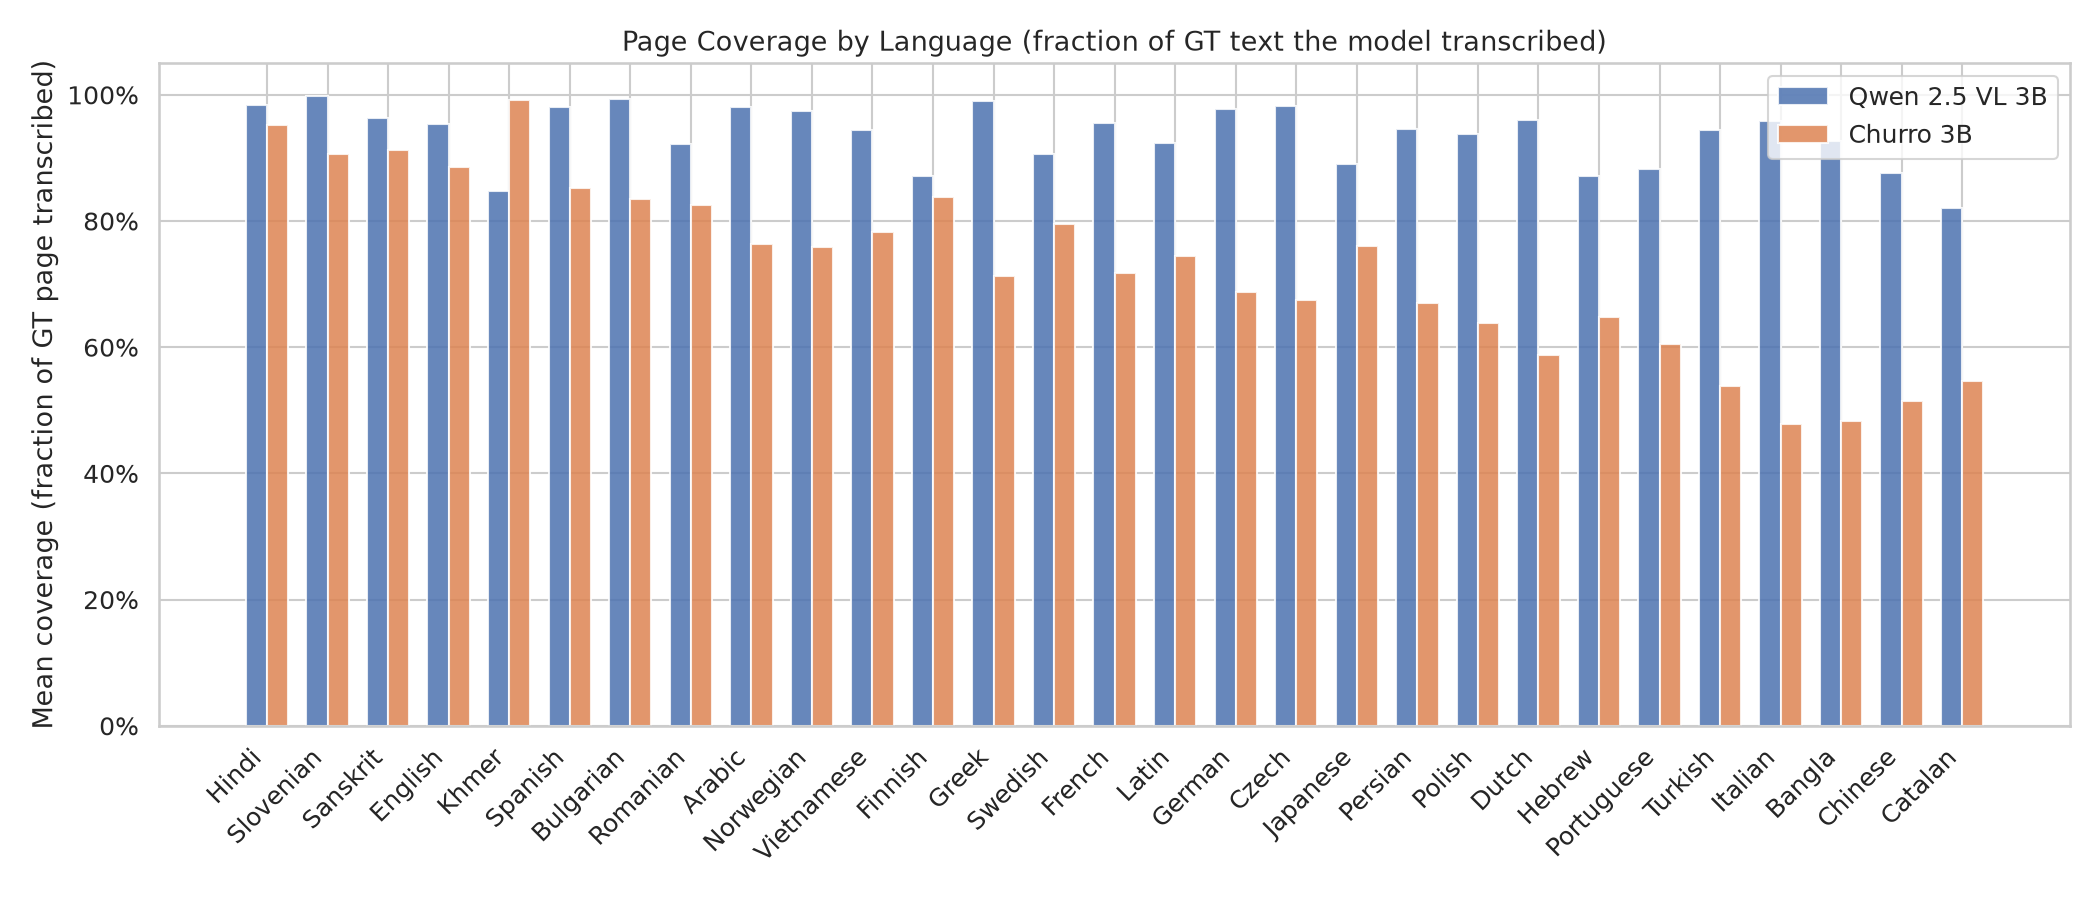
\includegraphics[width=\linewidth]{figures/01_coverage_by_language.png}
  \caption{Page coverage by language---fraction of the GT page each model transcribed.
    Stanford OVAL's Churro fine-tuning introduces a truncation tendency, most pronounced for
    CJK scripts and several European languages.}
  \label{fig:coverage}
\end{figure}

\begin{figure}[H]
  \centering
  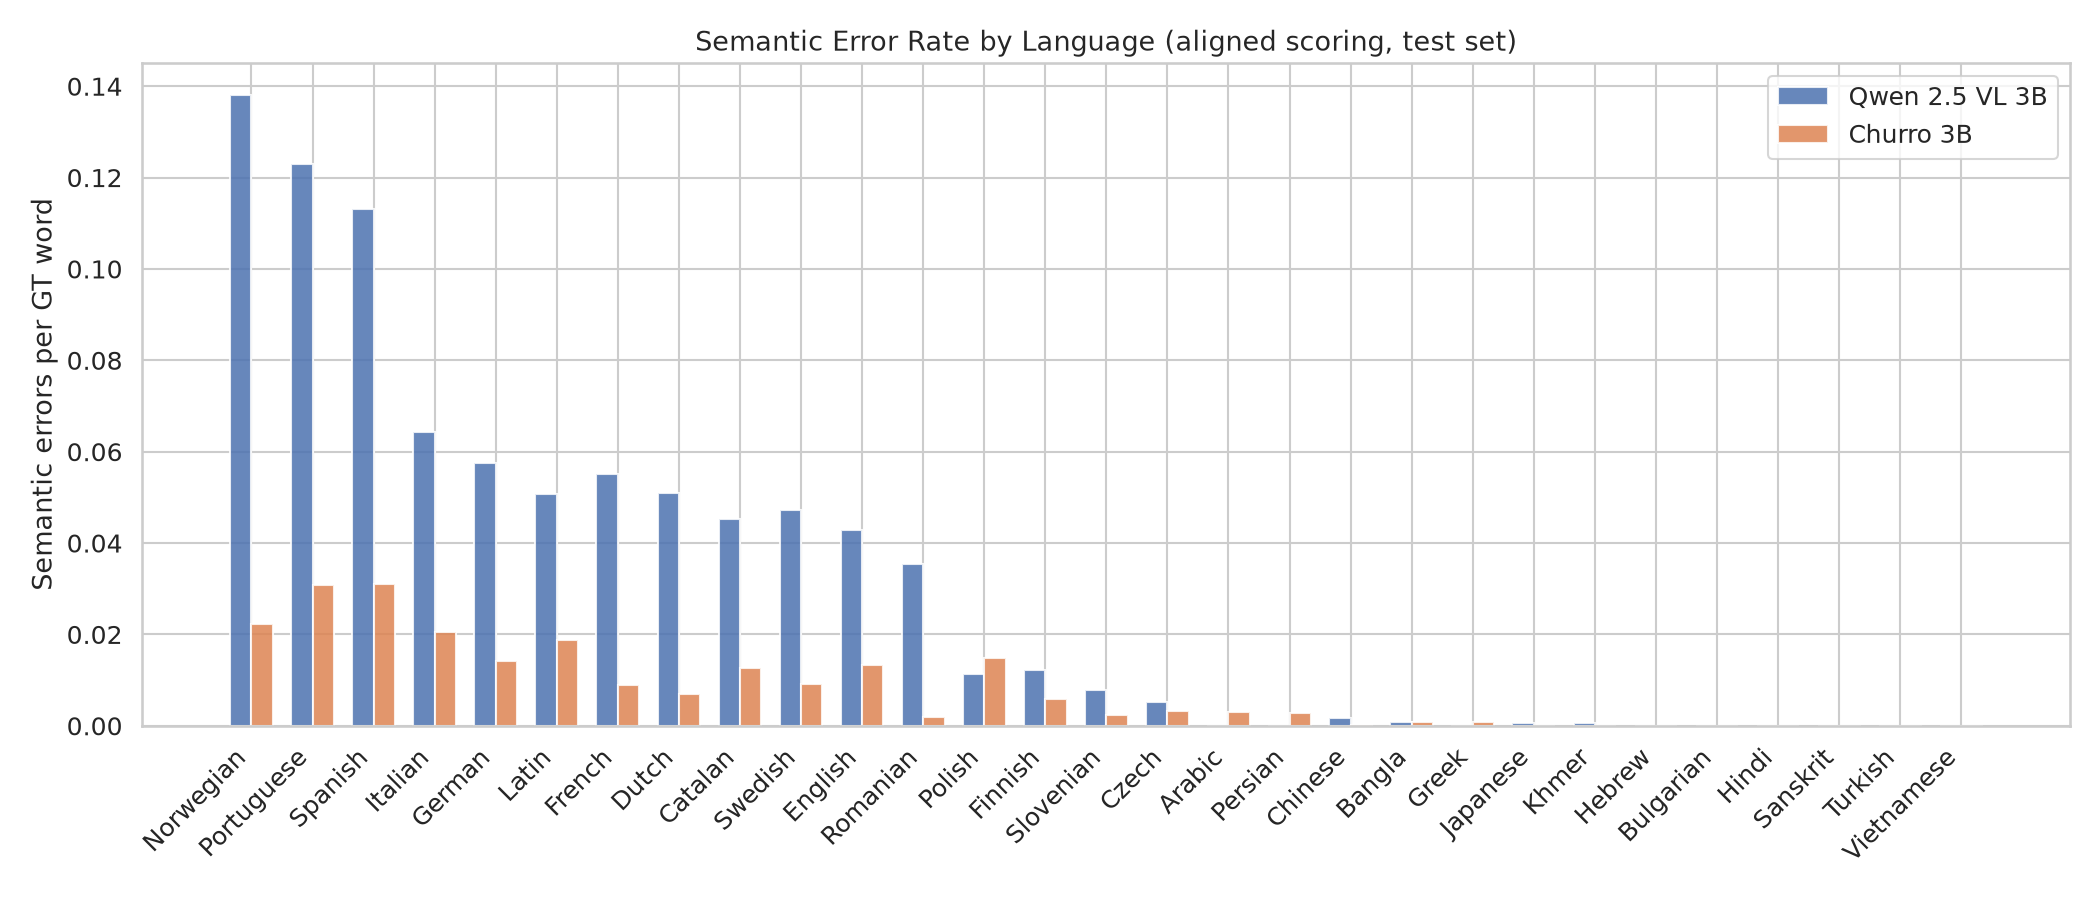
\includegraphics[width=\linewidth]{figures/03_semantic_error_by_language.png}
  \caption{Semantic error rate by language (errors per GT word, aligned scoring).
    Metrics are computed against the GT region each model actually covered,
    so this reflects transcription quality independent of coverage.}
  \label{fig:semantic}
\end{figure}

\section*{Semantic Errors per GT Word: Qwen vs.\ Churro}

$\Delta = \text{Churro} - \text{Qwen}$ (negative = fine-tuning reduced errors).
Mean $\Delta = -0.0220$; the final column shows
how each language deviates from that average shift.

\begin{table}[H]
\centering
\small
\begin{tabular}{lrrrr}
\toprule
Language & Qwen & Churro & $\Delta$ & $\Delta - \bar{\Delta}$ \\
\midrule
    Norwegian & 0.1381 & 0.0222 & -0.1160 & -0.0939 \\
    Portuguese & 0.1229 & 0.0308 & -0.0921 & -0.0700 \\
    Spanish & 0.1131 & 0.0311 & -0.0820 & -0.0599 \\
    French & 0.0551 & 0.0090 & -0.0462 & -0.0241 \\
    Dutch & 0.0509 & 0.0070 & -0.0439 & -0.0218 \\
    Italian & 0.0643 & 0.0206 & -0.0437 & -0.0217 \\
    German & 0.0575 & 0.0142 & -0.0433 & -0.0212 \\
    Swedish & 0.0473 & 0.0092 & -0.0381 & -0.0161 \\
    Romanian & 0.0353 & 0.0018 & -0.0335 & -0.0115 \\
    Catalan & 0.0452 & 0.0126 & -0.0326 & -0.0106 \\
    Latin & 0.0508 & 0.0188 & -0.0320 & -0.0100 \\
    English & 0.0428 & 0.0134 & -0.0295 & -0.0074 \\
    Finnish & 0.0121 & 0.0058 & -0.0064 & +0.0157 \\
    Slovenian & 0.0078 & 0.0023 & -0.0055 & +0.0166 \\
    Czech & 0.0051 & 0.0033 & -0.0018 & +0.0202 \\
    Chinese & 0.0017 & 0.0002 & -0.0015 & +0.0206 \\
    Japanese & 0.0007 & 0.0000 & -0.0007 & +0.0214 \\
    Khmer & 0.0006 & 0.0000 & -0.0006 & +0.0214 \\
    Vietnamese & 0.0000 & 0.0000 & +0.0000 & +0.0220 \\
    Turkish & 0.0000 & 0.0000 & +0.0000 & +0.0220 \\
    Hindi & 0.0000 & 0.0000 & +0.0000 & +0.0220 \\
    Bulgarian & 0.0000 & 0.0000 & +0.0000 & +0.0220 \\
    Sanskrit & 0.0000 & 0.0000 & +0.0000 & +0.0220 \\
    Hebrew & 0.0000 & 0.0000 & +0.0000 & +0.0220 \\
    Bangla & 0.0007 & 0.0007 & +0.0000 & +0.0220 \\
    Greek & 0.0000 & 0.0009 & +0.0009 & +0.0229 \\
    Persian & 0.0000 & 0.0029 & +0.0029 & +0.0249 \\
    Arabic & 0.0000 & 0.0029 & +0.0029 & +0.0249 \\
    Polish & 0.0113 & 0.0149 & +0.0036 & +0.0256 \\
\midrule
    \textbf{Mean} & 0.0298 & 0.0077 & -0.0220 & --- \\
\bottomrule
\end{tabular}
\caption{Semantic error rate (errors/GT word) by language, sorted by $\Delta$.
  $\Delta < 0$ indicates fine-tuning reduced semantic errors;
  $\Delta - \bar{\Delta} < 0$ indicates the language improved more than average.}
\label{tab:delta}
\end{table}

\end{document}
